\chapter{The SALSA website}
The SALSA telescopes have their own website at {\bf http://vale.oso.chalmers.se/salsa},
a part of the page can be sen in Fig. \ref{fig:website}. 
Here you can find a lot of useful information and software to assist you when using
the telescope and analysing data. 
\begin{figure}[h]
\centering
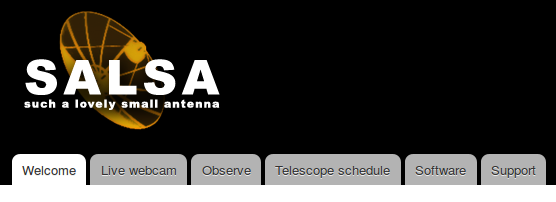
\includegraphics[width=\textwidth]{../figures/SALSA_website.png}
\caption{\label{fig:website} A part of the SALSA website. Here you find a
	lot of useful information as well as the booking system used to reserve
	observing time with SALSA.}
\end{figure}

\section{Create an account}
To be able to control the telescopes you need to 
register on the SALSA website. If you have not already, please find the link 
\emph{Create new account} and fill in your details. You should now get an email
confirmation with login information, if not - please check your spam filter.

\section{Book observing time}
To be able to observe you first have to book observing time. This is required
to ensure that only one user may control a SALSA telescope at any given time.
Bookings are made via the SALSA website. Once you are logged in with your
account, go to the page \emph{Observe}. On this page you find a link to
\emph{Book a time}. Click here to make a new reservation.  A new
page appears where you need to enter a \emph{brief description} of your
observation, see Fig. \ref{fig:book}.
\begin{figure}[h]
\centering
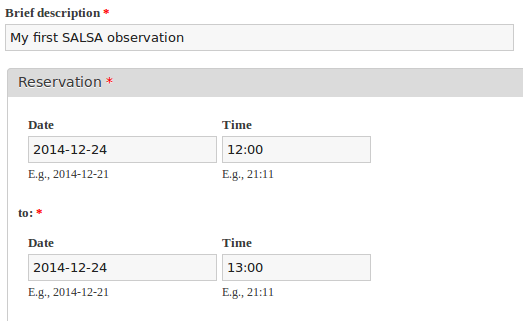
\includegraphics[width=\textwidth]{../figures/SALSA_book.png}
\caption{\label{fig:book} The page used to create a new reservation, i.e.
	book observing time with SALSA.}
\end{figure}

Then, select start and end times of your observation. (You may want to check
the page \emph{Telescope schedule} to find a suitable time.)  Note that you may
click in the date-fields to get a pop-up calendar where you can select a day.
The time fields specify hours and minutes on the selected day. Note that you
can switch from editing hours to minutes by clicking with the mouse or using
the right and left arrow-keys on your keyboard. Note that times are displayed
in the timezone you selected when registering. (If you want to check or change
your timezone, click on \emph{My account}.)

Finally you need to chose a telescope. We try to always have at least one
telescope available, but sometimes there are two or three telescopes available.
They are booked independently, so if one telescope is booked at a certain time
you can select another.  Select at least one telescope and then press
\emph{Save} to save your reservation.  You should now see your reservation on
the page \emph{My reservations}, as well as on the page \emph{Telescope
schedule}. You will now be able to control the telescope you booked during your
reserved time. Note that you cannot access the telescopes if you have not
booked. Note also that should your reservation end while you are observing,
your observations will be terminated. Please make sure to save your data while
observing, see below, and do not leave it to the end. If you realise while
observing that you will require more time, you can try to extend your
reservation. This can be done on the page \emph{My reservations}: just use the
link \emph{edit} to change a specific reservation.

\section{Live webcam}
It is much more fun to move telescopes if you can see them move! Therefore
we have put a camera in a nearby building which you can access through the 
page \emph{Live webcam} on the SALSA website.

\section{Online data archive}
\label{sect:archive}
When you have made a measurement with SALSA you can upload save it to an online
archive. To access your archived data, log in to the SALSA website and click
the link \emph{Data archive}. This page displays your personal archive, showing
all your saved observations.  Each measurement can be downloaded as three
different formats: as PNG (an image, convenient for a quick look at your
measurement), as TXT (a plain text file with the raw numbers), and as FITS 
(a common data format in astronomy to inspect the data in great detail).
Instructions on how to read the data in these formats are given in Sect.
\ref{sect:archiveprocess}.
\begin{figure}[h]
\centering
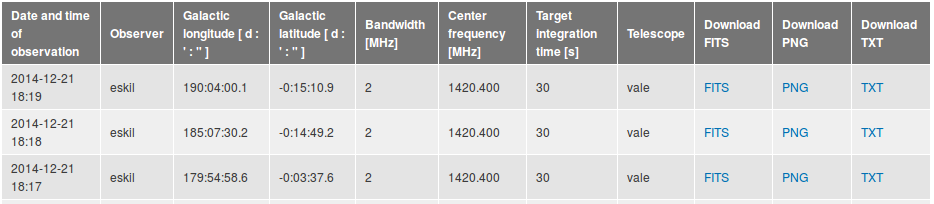
\includegraphics[width=\textwidth]{../figures/SALSA_archive.png}
\end{figure}
